\documentclass[12pt]{article} % use larger type; default would be 10pt

\usepackage{tikz}
\usetikzlibrary{positioning, automata}
\usetikzlibrary{trees}

\begin{document}

Test graph 2
\\ V1: Position: A speed: 2
\\ V2: Position: C speed: 3
\\
r1 A--B timestep: 0
\\ r2 D--B timestep: 0
\\ r3 B--C timestep: 1
\\r4 A--C timestep: 3 

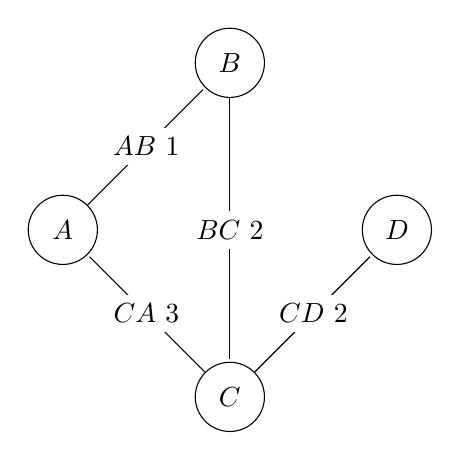
\begin{tikzpicture}[shorten >=1pt,node distance=3cm,on grid,initial/.style    ={}]
  \node[state]          (A)                        {$A$};
  \node[state]          (B) [above right =of A]    {$B$};
  \node[state]          (C) [below right =of A]    {$C$};
  \node[state]          (D) [below right =of B]    {$D$};
\tikzset{mystyle/.style={-}} 
\tikzset{every node/.style={fill=white}} 
\path (A)     edge [mystyle]    node   {$AB\ 1$} (B)
      (C)     edge [mystyle]    node   {$CA\ 3$} (A) 
      (B)     edge [mystyle]    node   {$BC\ 2$} (C)
      (C)     edge [mystyle]    node   {$CD\ 2$} (D);
\end{tikzpicture}

\bigskip

Test graph 1
\\ V1: Position: A speed: 1
\\ V2: Position: D speed: 1
\\
r1 C--A timestep: 0
\\ r2 D--E timestep: 1

\begin{tikzpicture}[shorten >=1pt,node distance=3cm,on grid,initial/.style    ={}]
  \node[state]          (A)                        {$A$};
  \node[state]          (B) [right =of A]    {$B$};
  \node[state]          (C) [right =of B]    {$C$};
  \node[state]          (D) [below =of C]    {$D$};
 \node[state]          (E) [right =of C]    {$E$};
\tikzset{mystyle/.style={-}} 
\tikzset{every node/.style={fill=white}} 
\path (A)     edge [mystyle]    node   {$AB\ 4$} (B)
      (C)     edge [mystyle]    node   {$CB\ 4$} (B) 
      (D)     edge [mystyle]    node   {$DC\ 4$} (C)
      (E)     edge [mystyle]    node   {$EC\ 4$} (C);
\end{tikzpicture}

\begin{tabular}{l|l|l|l}
& graph no. & avg. wait time & unoccupied travelled\\ \hline
Stupid & 1 & 54 & 390\\ 
 & 2 & 290 & 903\\
 & 3 & ? & ?\\ \hline
Basic SCRAM & 1 & 24 & 216\\ 
 & 2 & 106 & 472\\
 & 3 & ? & ?\\ \hline
w. extension 1 & 1 & ? & ?\\ 
 & 2 & ? & ?\\
 & 3 & ? & ?\\ \hline
Extension 2 & 1 & ? & ?\\
 & 2 & ? & ?\\
 & 3 & ? & ?\\
\end{tabular}

\end{document}